\documentclass[a4paper,oneside,twocolumn,notitlepage,dvipdfmx]{jsarticle}
\usepackage[utf8]{inputenc}
\usepackage{amsmath}
\usepackage{amsfonts}
\usepackage{amssymb}
\usepackage{makeidx}
\usepackage{graphicx}
\usepackage{color}
\usepackage{sample}
\usepackage{url}
\usepackage{listings,jlisting}
\setlength\abovecaptionskip{1pt}
\def\baselinestretch{0.3}


\lstset{
  basicstyle={\ttfamily},
  identifierstyle={\small},
  commentstyle={\smallitshape},
  keywordstyle={\small\bfseries},
  ndkeywordstyle={\small},
  stringstyle={\small\ttfamily},
  frame={tb},
  breaklines=true,
  columns=[l]{fullflexible},
  numbers=left,
  xrightmargin=0zw,
  xleftmargin=3zw,
  numberstyle={\scriptsize},
  stepnumber=1,
  numbersep=1zw,
  lineskip=-0.5ex
}

% 以下内容

\student{谷澤 悠太}
\date{令和5年12月21日}
\prof{滝沢 寛之}
\title{中間報告}
%\author{Maohua Zhu, Tao Zhang, Zhenyu Gu, Yuan Xie}
%\journal{MICRO-52, October 12-16, 2019, Columbus, OH, USA}
\nendo{令和5年度}

\begin{document}
\maketitle
\section{背景}
HPCは現在,機械学習や数値シュミレーション,統計解析など様々な科学分野で地擁されている.そのため,HPCを専門としない科学者がHPCを利用する事例や情報系学生などがHPCを用いた並列計算を学習する際に利用するといった事例が多く存在する.しかしながら,このような事例の場合,HPC利用のための環境構築や鍵認証のためのセットアップが諸学者にとって複雑であることやCLIベースでスケジューラなどに命令を出すことの難易度の高さなどが利用者にとって障害となる.このことは,HPCを使いこなすための学習コストの大きさにより,本来の研究に費やすコストが減少してしまうため問題となっている.\par
このような問題に対して,米国オハイオ・スーパーコンピューティングセンターはHPC利用者の支援を目的とする『Open OnDemand』(OOD)と呼ばれるオープンソースソフトウェアを開発した.\cite{citation_3}\cite{citation_4}\cite{citation_5}OODはWebポータル上からHPCシステムの利用を可能としており,CLIではなくGUIベースで操作することが可能なため,初学者に寄り添ったHPC利用環境を提供することができる.また,ユーザ情報の登録によるシングルサインオン認証を用いることで,誰でも環境構築を行わずに利用することが可能となっている.開発当時のOODはSLURM,Torque,PBS Pro,LSFなどのジョブスケジューラに対応していたため,現在OODを導入している計算センターも多く存在する.しかしながら,対応していないスケジューラも多く,使える環境が限定されているといえる.\par
そこで先行事例として,OODをFujitsu\_TCS(スーパーコンピュータ富岳で運用されているジョブスケジューラ)へ対応させたことによる『富岳』でのOOD利用という事例を考える.\cite{citation_1}これにより,『富岳』の利用者はHPCシステムの視覚的理解が容易になった,利用難易度が低下した,などのメリットを得ることができた.また,Fujitsu\_TCSのアダプタの開発により,Fujitsu\_TCSを利用している他の計算センターでもOODの利用が可能となったというメリットもある.\par

\section{目的}
本研究では『ウェブインタフェースを介したスーパーコンピュータ利用環境に関する研究』という題目を研究テーマとして考えていく.具体的には,東北大学で用いられているスーパーコンピュータ『AOBA』の利用環境について考える.前述の通り,OODはいくつかのジョブスケジューラに対応しているが,『AOBA』に用いられているジョブスケジューラNQSV(Network Queuing System V)に対応するためのアダプタが存在しない.そのため,NQSVのアダプタを実装することでAOBA利用者の支援を目的とする.\par

\section{実装手順}
具体的な実装について,大きく4つの手順に分けて紹介する.\par
まず, 1つ目の手順としてSLURMスケジューラを試用しているsendaiサーバでOODの動作確認を行う.この手順でOODがどのようなものか理解したり,システムの設計について調査し,具体的な実装手順を見据える.\par
2つ目の手順として,SLURM用に書かれたアダプタファイルを自分で書き換えることでOODにその変更内容が反映されるかどうかを確認する.\par
3つ目の手順として,tokyo,paris,londonの3つのサーバにNQSVをインストールしてAOBAのテスト環境を構築する.\par
4つ目の手順として,他のスケジューラのアダプタを参考にしてNQSVのアダプタを作成する.このとき,NQSVと親和性の高いPBS Proや動作確認で試用したSLURM,アダプタ作成例が紹介されているFujitsu\_TCSのアダプタなどを参考にする.\par
最後の手順として,手順2や手順3の過程からアダプタの構造理解やその汎用性などの検討を行う.アダプタやスケジューラの理解を深めることで,様々なスケジューラに対応できる汎用性の高いアダプタについて考察したい.

\section{進捗}

\subsection{テスト環境構築手順}
現在の進捗として,手順3で示したAOBAのテスト環境構築が終了している.以降にテスト環境の詳細を示す.\par
テスト環境の構築は大きく3つのステップで手順が実行さてていく.1ステップ目がOSのインストール,2ステップ目が3つのサーバへのNQSVのインストール,3つ目が各コンポーネントの設定である.\par

\subsection{OSインストール}
使用するtokyo,london,parisにUbuntu22.04.3 LSTが入っていたがNQSVはUbuntuに対応していないため,NQSVの動作確認が保証されているCentOS7を導入した.OSのインストールにはboot起動用のUSBを作成し,各種設定を行った.\par
最初に,rikenのミラーサイトからCentOS7の実体をインストールしてrufusというアプリケーションを用いてboot起動用のUSBを作成した.各種設定として,言語選択,時刻選択,Software選択,インストール先選択,rootユーザのパスワード設定などを行った.また,ネットワークとホスト名設定に関して,もともと各サーバに割り当てられていらIPアドレスとホスト名を設定した.また,研究室で用いているADとの連携,ファイルシステムの同期が必要だったため,localwikiを参考に,ADとの連携と,cieroのホームディレクトリと連携するためのNFSの設定を行った.\par

\begin{figure}[h]
  \centering
  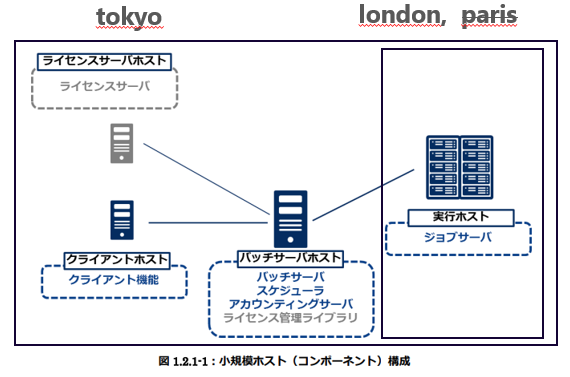
\includegraphics[width=75mm]{/home/gp.sc.cc.tohoku.ac.jp/tanizawa/study_session/2022/3rd_latex/preprint/20231221/fig/fig_1.png}
  \caption{AOBAテスト環境のホスト構成}
  \label{fig_1}
\end{figure}

\subsection{NQSVのインストール}
AOBAテスト環境のホスト構成を図\ref{fig_1}に示す.今回のテスト環境ではtokyoをマスターノードとしてスケジューラやNQSV全体の管理を担うものとする.また,tokyo,london,parisに実行ホストをおいてジョブの割り当てを行う.\par
ここでホスト構成に示した各ホストの役割を説明する.ライセンスサーバホストは,ライセンス製品の利用に必要なライセンスの管理を行う.バッチサーバホストにはバッチサーバ,スケジューラ,アカウンティングサーバが置かれ,バッチサーバがNQSVの中心コンポーネントであり,スケジューラがジョブリクエストの管理を行い,アカウンティングサーバではアカウント管理や,予算管理を行う.また,クライアントホストはリクエストの投入やNQSV全体の管理操作を行う.これらの3つのホストは今回のテスト環境ではすべてtokyo上に設置することとする.また,各サーバに置く実行ホストは,各サーバのジョブ実行の管理をする.\par



\subsubsection{ライセンスサーバの設定}
JobServer(ジョブサーバ)とJobManipulator(スケジューラ)の仕様にライセンスが必要であるため,まずはじめにtokyoのライセンスサーバの設定を行う.ライセンスサーバ(aurlic-lib)のインストールを行った後,ファイヤーウォールの設定でポート7300番を開けておく.その後ライセンスサーバを起動する.\par
また,ライセンスのクライアント側として,今回使用するすべてのマシン上にライセンスアクセスライブラリをインストールする.、また,各マシンで設定ファイル(\texttt{/opt/nec/aur\_license/aur\_license.conf})にホスト名を登録してライセンスサーバの情報を登録する.\par

\subsubsection{NQSVメインコンポーネントインストール}
NQSVのメインコンポーネントを各サーバホストにインストールする.ライセンスサーバは無償のトライアル提供があったが,こちらは有償ソフトウェアであったため下村先生経由でいただいたものをインストールした.バッチサーバホスト、アカウンティングサーバホスト、運用管理ホストであるtokyoにNQSV-ResourceManagerをインストールする.また,クライアントホスト,バッチサーバホストであるtokyoにNQSV-Client,NQSV-JobManipulatorをインストールする.最後に各実行ホストにNQSV-JobServerをインストールして主なコンポーネントのインストールが完了する.

\subsubsection{バッチサーバの設定}
まず始めに,バッチサーバのユニット(nqs-bsv)の起動を行う.続いて,バッチサーバホストに任意のマシンIDを登録してデータベースを初期化する.その後,nqs\_bsvdコマンドを用いてバッチサーバを起動,ユーザマップファイル(/etc/opt/nec/nqsv/nqs\_user.map)にユーザと権限を登録する.\par

\subsubsection{クライアントホスト設定}
クライアントホストであるtokyo上の設定ファイル(/etc/opt/nec/nqsv/api\_client.conf)にバッチサーバホスト名を記述する.また同じく,tokyo上の設定ファイル(/etc/opt/nec/nqsv/nqs\_jmd\_cmdapi.conf)にスケジューラホスト名を記述する.これらの設定により,クライアントホストの環境設定が完了した.\par

\subsubsection{実行ホスト設定}
まず,実行ホスト上でqmgrコマンドとattach\ execution\_hostサブコマンドを用いて実行ホストとジョブサーバ番号を指定する.次に,各事項ホストでランチャーデーモン(nqs-lchd)を起動する.最後に,qmgrコマンドのstart job\_server allコマンドですべてのジョブサーバを起動して実行ホストの設定を完了する.\par
図\ref{fig_2}に示すようにqstat -Etコマンドを用いて各実行ホストのステータスを確認することができる.JSVNO(ジョブサーバ番号)が0のものがtokyoで,1のものがlondonになっている.どちらのサーバも接続状態(LINK UP)になっており正常に動作していることがわかる.

\begin{figure}[h]
  \centering
  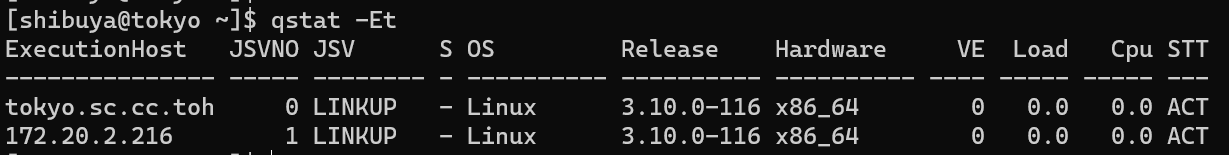
\includegraphics[width=75mm]{/home/gp.sc.cc.tohoku.ac.jp/tanizawa/study_session/2022/3rd_latex/preprint/20231221/fig/fig_2.png}
  \caption{各実行ホストのステータス}
  \label{fig_2}
\end{figure}

\subsubsection{スケジューラ設定}
まず,インストールしたJobManipulatorを起動する.続いて,smgr -Poコマンドでstart schedulingを指示してスケジューリングを開始する.\par

\subsubsection{キュー設定}
qmgrコマンドのcreate execution\_queueサブコマンドを使用して,キューの名前(execque1)とキューのプライオリティを指定してキューを作成する.続いて,bind execution\_queue job\_server サブコマンドを用いてキュー名とジョブサーバ番号を指定することで,バッチキューとジョブサーバをバインドする.さらに,bind execution\_queue scheduler サブコマンドを用いて,キュー名とスケジューラのIDを指定することで,バッチキューとスケジューラをバインドする.最後に,enable execution\_queue サブコマンドとstart execution\_queue サブコマンドによってバッチキューを開始する.\par
図\ref{fig_3}に示すようにqstat -Qeコマンドを用いてバッチキューのステータスを確認することができる.4列目,5列目のENA,STSがキューのステータスを表していて,それぞれenable,activeとなっていて正常に動作していることがわかる.\par

\begin{figure}[h]
  \centering
  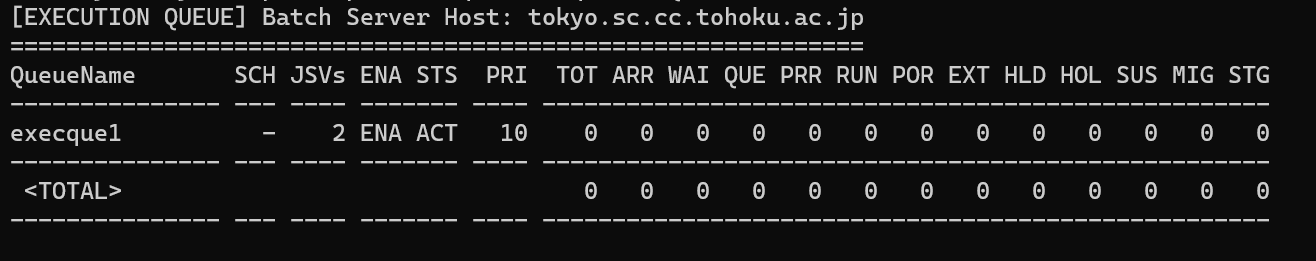
\includegraphics[width=75mm]{/home/gp.sc.cc.tohoku.ac.jp/tanizawa/study_session/2022/3rd_latex/preprint/20231221/fig/fig_3.png}
  \caption{バッチキューのステータス}
  \label{fig_3}
\end{figure}

\subsubsection{アカウンティングサーバ設定}
アカウンティングサーバ(nqs-asv)とアカウンティングモニタ(nqs-acm)の起動を行う.続いて,予約管理機能について設定ファイル(/etc/opt/nec/nqsv/asvd.conf)において$SBU\_CHECK=ON$とする.また,バッチサーバ側の環境設定として,バッチサーバ上でqmgr -Pmコマンドを用いて予算管理機能,リソース予約区間に対する課金設定,リクエストアカウントとジョブアカウントの設定,アカウンティングサーバ情報の設定を行った.

\subsubsection{リクエスト実行の確認}

\begin{verbatim}
  qsub -q execque1 -l elapstim_req=200 --cpunum-
  lhost=1
  uname -a
  sleep 100
\end{verbatim}

とコマンドを打つことでキューにリクエストを投入する.投入状態はqstatコマンドで確認することができ,図\ref{fig_4}にqstatの出力結果を示す.ジョブの100秒間のスリープをリクエストしたため,ステータスはRunning状態になっていて,経過時間も100秒間経つまで増加していることがわかる.\par

\begin{figure}[h]
  \centering
  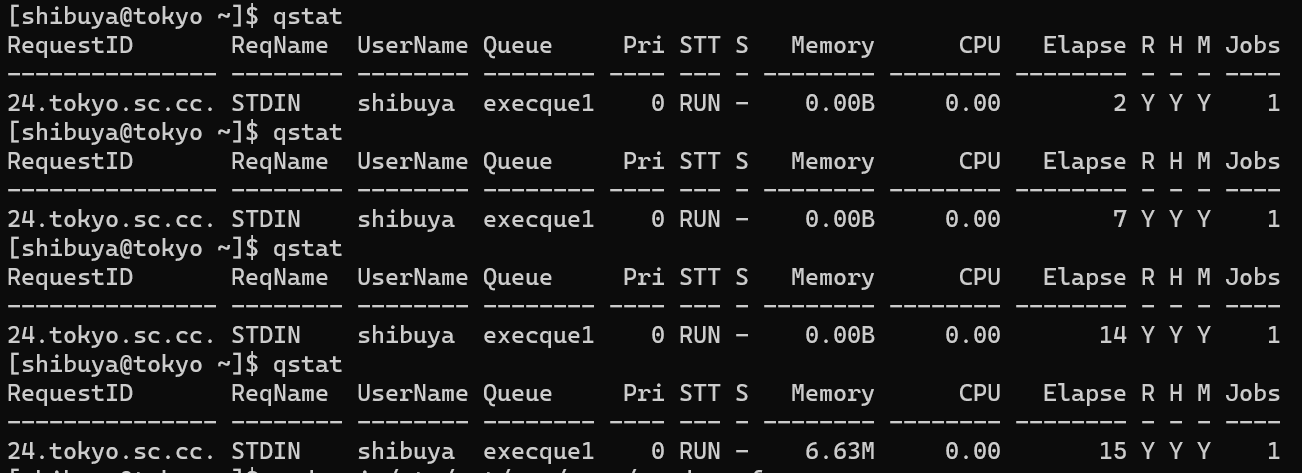
\includegraphics[width=75mm]{/home/gp.sc.cc.tohoku.ac.jp/tanizawa/study_session/2022/3rd_latex/preprint/20231221/fig/fig_4.png}
  \caption{qstat出力結果}
  \label{fig_4}
\end{figure}

\section{今後の予定}
短期目標として,\par
・テスト環境の整備\par
・コマンドの出力形式をAOBAと一致させる\par
\qquad・NQSVのアダプタを書き始める\par
中長期目標として,\par
・SSHFSを用いたOOD経由のリモートHPCクラスタへのジョブ投下について検討\par
・卒論構成についての深掘り\par
を考えている.\par

\bibliographystyle{junsrt}
\bibliography{refer}

\end{document}